\documentclass[tikz,border=1pt]{standalone}

\usepackage{amsmath}
\usepackage{xcolor}
\usepackage{pifont}
\usepackage{fontspec}
\usepackage{unicode-math}

\setsansfont{DejaVu Sans}[ UprightFont = DejaVu Sans, ItalicFont = DejaVu Sans Oblique, BoldFont = DejaVu Sans Bold, BoldItalicFont = DejaVu Sans Bold Oblique ]
\setmathfont{TeX Gyre DejaVu Math}
\renewcommand{\familydefault}{\sfdefault}

\definecolor{allowedgreen}{RGB}{0,175,90}
\definecolor{forbiddenred}{RGB}{230,0,55}

% One horizontal level
\newcommand{\singlelevel}[3]{%
    \draw[level] (#1-0.35,#2) -- (#1+0.35,#2);
    \node at (#1,#2+0.00) {\huge$#3$};
}

\newcommand{\singleleveltwo}[4]{%
    \draw[level] (#1-0.35,#2) -- (#1+0.35,#2);
    \node at (#1-0.1,#2+0.00) {\huge$#3$};
    \node at (#1+0.1,#2+0.00) {\huge$#4$};
}

% Two adjacent horizontal levels
\newcommand{\doublelevel}[4]{%
    \draw[level] (#1-0.80,#2) -- (#1-0.15,#2);
    \draw[level] (#1+0.15,#2) -- (#1+0.80,#2);
    \node at (#1-0.475,#2+0.00) {\huge$#3$};
    \node at (#1+0.475,#2+0.00) {\huge$#4$};
}

% Allowed and forbidden marks
\newcommand{\allowed}[2]{%
    \node[text=allowedgreen,font=\bfseries\fontsize{20}{20}\selectfont]
    at (#1,#2) {\ding{51}};
}

\newcommand{\forbidden}[2]{%
    \node[text=forbiddenred,font=\bfseries\fontsize{24}{24}\selectfont]
    at (#1,#2) {$\boldsymbol{\times}$};
}

\begin{document}

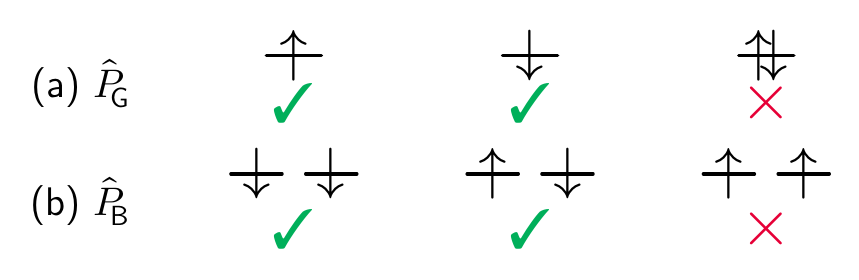
\begin{tikzpicture}[
    line cap=round,
    line join=round,
%    every node/.style={font=\large},
%    every node/.style={font=\large,inner sep=1pt,outer sep=1pt},
%    every node/.style={font=\sffamily\large,inner sep=1pt,outer sep=1pt},
    every node/.style={font=\sffamily\Large,inner sep=1pt,outer sep=1pt},
    level/.style={draw=black,line width=1.2pt}
]

% (a) Gutzwiller projector
\node[anchor=east] at (-2.0,1.65) {\textnormal{(a)} $\hat{P}_{\!\!\textnormal{G}}$};

\singlelevel{0.0}{2.00}{\boldsymbol{\uparrow}}
\allowed{0}{1.40}

\singlelevel{3.0}{2.00}{\boldsymbol{\downarrow}}
\allowed{3.0}{1.40}

\singleleveltwo{6.0}{2.00}{\boldsymbol{\uparrow}}{\boldsymbol{\downarrow}}
\forbidden{6.0}{1.40}

% (b) Blockade projector
\node[anchor=east] at (-2.0,0.15) {\textnormal{(b)} $\hat{P}_{\!\!\textnormal{B}}$};

\doublelevel{0}{0.50}{\boldsymbol{\downarrow}}{\boldsymbol{\downarrow}}
\allowed{0}{-0.20}

\doublelevel{3.0}{0.50}{\boldsymbol{\uparrow}}{\boldsymbol{\downarrow}}
\allowed{3.0}{-0.20}

\doublelevel{6.0}{0.50}{\boldsymbol{\uparrow}}{\boldsymbol{\uparrow}}
\forbidden{6.0}{-0.20}

\end{tikzpicture}

\end{document}
